\documentclass[12pt,oneside]{memoir} 
\usepackage[latinica]{matfmaster}
\usepackage[latinica]{pangrami}
\usepackage{mathtools}
\usepackage{amsmath}
\usepackage{fixltx2e}
\usepackage{graphicx}
\usepackage{url}


% Datoteka sa literaturom u BibTex tj. BibLaTeX/Biber formatu
%\bib{Master_rad}

\autor{Ljubica Peleksić}
\naslov{Klasifikacija obolelih od Alchajmerove bolesti na osnovu analize spontanog govora}
\godina{2021}

\mentor{doc. dr Jelena Graovac, profesor\\ Univerzitet u Beogradu, Matematički fakultet}

% Dodati clanove komisije i datum odbrane
\komisijaA{prof. dr Gordana Pavlović-Lažetić}
\komisijaB{doc. dr Jovana Kovačević}
\datumodbrane{}

% Apstrakt na srpskom jeziku (u odabranom pismu)
\apstr{%
% TODO Dodati apstrakt
}


% Ključne reči na srpskom jeziku (u odabranom pismu)
\kljucnereci{klasifikacija, Alchajmer, NLP}

\begin{document}

% ==============================================================================
% Uvodni deo teze
\frontmatter
% ==============================================================================
% Naslovna strana
\naslovna
% Strana sa podacima o mentoru i članovima komisije
\komisija
% Strana sa posvetom (u odabranom pismu)
% TODO Dodati posvetu
\posveta{porodici}
% Strana sa podacima o disertaciji na srpskom jeziku
\setsecnumdepth{subsection}

% Sadržaj teze
\tableofcontents{}

% ==============================================================================
% Glavni deo teze
\mainmatter
% ==============================================================================

% ------------------------------------------------------------------------------

\chapter{Uvod}

Alchajmerova bolest je najčešći oblik demencije koja uzrokuje probleme sa pamćenjem,  mišljenjem,  govorom i ponašanjem.  Simptomi se obično razvijaju polako i vremenom se pogoršavaju do te mere da obolelim osobama znatno mogu ometati obavljanje svakodnevnih zadataka.  Dešavaju se kada su neuroni u delovima mozga koji su zaduženi za učenje i memoriju, tj. kognitivne funkcije oštećeni. \cite{Alzheimerfactsfigures}.  Najraniji simptom je otežano pamćenje novih informacija, a zatim nastupaju poteskoće u govoru i gubitak memorije.  Kasnije u toku bolesti se pojavljuju i problemi pri obavljaju nekih jednostavih zadataka,  gubitak sposobnosti da nastave razgovor i da reaguju na svoju okolinu,  vremenska i prostorna dezorijentacija.  Alchajmerova bolest ne predstavlja normalan deo starenja iako godine predstavljaju najizraženiji faktor rizika.  Oko 6 do 10\% ljudi preko 65 godina ima neki oblik demencije,  a 60 do 70\% tih ljudi ima upravo Alchajmerovu bolest.\cite{actavis} Svake tri sekunde u svetu neko razvije demenciju, a Alchajmerova bolest je najčešci oblik demencije.  Procenjuje se da danas oko 50 miliona ljudi u svetu imaju Alchajmerovu bolest ili demenciju vezanu za nju.  Pretpostavlja se da bi ovaj broj mogao da naraste do 82 miliona do 2030.  godine. i do 152 miliona do 2050. godine.  \cite{Languageimpairment}.  U proseku, osoba sa Alchajmerovom bolešću živi četiri do osam godina nakon dijagnoze,  ali može da živi i do 20 godina, u zavisnosti od drugih faktora \cite{seracell}. 

Tačan uzork bolesti nije poznat,  ali se pretpostavlja da učestvuje više udruženih faktora kao što su genetski činioci, ranija oboljenja, uticaj životne sredine i promene na mozgu uzrokovane starenjem \cite{medicor}.

Metodi za dijagnostifikovanje bolesti se sastoje iz struktuiranih intervjua koje izvode lekari.  Tokom ovih intervjua je teško da se  uoči kompleksna priroda nedostataka koji se mogu naći u govoru obolele osobe.  

Ovi intervjui testiraju jezičke sposobnosti i uključuju imenovanje objekata,  izgovaranje jedne reči,  generisanje reči iz datog konteksta ili generisanje reči sa određenim početnim slovom.\cite{automaticdetandrat}.  Dijagnostifikovanje Alchajmerove bolesti je najlakše iz ugla porodice i prijatelja,  pošto su oni u stanju da u svakodnevnom životu,  pri normalim konverzacijama,  primete male promene u ponašanju bližnjih. 

Teži se automatizovanom pristupu sa objektivnim metodama dijanostifikovanja bolesti,  kao i određivanja stepena progresije.  Ovakav novi pristup je neophodan kako zbog preciznosti i zbog ranog dijagnostifikovanja bolesti,  tako i zbog brzine dobijanja dijagnoze i činjenice da bi time dijanozu i tretman za ublažavanje simptoma moglo dobiti više ljudi u svetu, među kojima danas mnogi nemaju pristup lekarima i lekarskoj nezi.  Takođe,  ovo bi omogućio dijanozu osobama sa izrazito napredom demencijom koje ne mogu da prolaze kroz psihološko testiranje.  Takođe,  automatizovan pristup bi doneo i mogućnost da se odredi nivo poboljšanja kod obolelog u toku ili nakon neke terapije ili leka\cite{Evaloftechfolexicalperformance}.

Zato tražimo metod za dijanostifikovanje koji je pouzdan,  objektivan,  lak za izvođenje i dovoljno precizan.

Prema Svetskom izvestaju o Alchajmeru iz 2011. godine postoje benefiti rane dijagnoze i intervencije koji su efektivniji u ranim stadijumima bolesti i omogućava osobama da isplaniraju negu i tretmane koje žele da imaju u budućnosti. Pored korišćenja lekova, a ima ih nekoliko,  smanjenje pogoršanja u kognitivnih funkcija osobe može pružiti i specijalizovana terapija. 

U više naučnih radova i studija je pokazano da korišćenjem obrade prirodnog jezika (eng. natural language processing) i mašinskog učenja (eng. machine learning) se može doći do vrednih podataka.  Motivacija za ovom vrstom obrade podataka i zaključivanja,  koji će biti predstavljeni u narednim poglavljima,  je nastala iz \cite{automaticdetandrat} i  \cite{linguisticfeatures}

Problem koji se rešava u okviru ovog rada je da li je moguce primeniti automatizaciju postupka dijagnostifikovanja obolelih od Alchajmerove bolesti dovoljno precizno, tačnije da li je moguće razlikovati starije subjekte od subjekata koji pate od  Alchajmerove bolesti na osnovu spontanog govora.  Ono što pojedinac izgovara je nepresušan izvor informacija o njemu samom,  a upravo tom činjenicom se vodimo kada vidimo mogućnost u nalaženju dijanoze analizom spontanog govora.  Dva pravca istraživanja su praćena,  jedan lingvistički i drugi putem metoda mašinskog učenja.  U sklopu lingvističkog pristupa,  određene,  već poznate metrike se izračunavaju za svaki intervju,  koji je predstavljen skupom reči,  njenom vrstom reči i lemom.  

U okviru ovog pristupa tražimo pravilnosti u govoru koje nam mogu pokazati da osoba boluje baš od ove bolesti.  U pristupu mašinskim učenjem ne postoje poznate metrike,  već se prepušta algoritmima da uoče zakonitosti u podacima u obliku učestalosti korišćenja reči i na taj način se preciziraju zakonitosti i razlike između dve grupe pacijenata. 

Do danas nije pronađen lek koji zaustavlja ili usporava razvoj bolesti, ali postoje lekovi za koje se smatra da mogu da uspore bolest ako je rano dijagnostifikovana, kao i oni za koje se smatra da poboljšavaju kognitivne funkcije obolele osobe.\cite{Alzheimerfactsfigures}.  Lekovi za demenciju mogu da uspore napredovanje bolesti u ranim i srednjim fazama.  Cilj lečenja Alchajmerove bolesti je što duže očuvanje sposobnosti i samostalnosti bolesnika i osim redovnog uzimanja lekova značajna je i primena drugih mera koje mogu značajno pomoći pacijentu\cite{medicor}.

Ovu temu razrađujemo kroz šest poglavlja, gde se nakon uvodnog poglavlja osvrćemo na podatke korišćene u praktičnom radu, način sakupljanja i obrade podataka.  U drugom poglavlju je opisan način rešavanja ovog problema metodama lingvističke analize,  gde su predstavljene metrike koje su korišćene kao i motivacija za njihov izbor. Treće poglavlje predstavlja prikaz rešavanja problema metodama mašinskog učenja,  modele reprezentacije teksta kao i algoritme mašinskog učenja koji su iskorišćeni u praktičnom radu.  U okviru petog poglavlja se diskutuju dobijeni rezultati reprezentativnog uzorka,  primenama svih metoda, dok se u poslednjem poglavlju,  u okviru zaključka,  sumiraju dobijeni rezultati i korišćene metode. 


\chapter{Podaci}

Kod rešavanja problema obradom prirodnih jezika, pored važnosti algoritama koji se koriste, treba istaći važnost podataka koji se predaju tim algoritmima.  Bez podataka,  algoritam sam nema nikavu vrednost.  Izazov je sam po sebi pronaći dovoljnu količinu podataka,  kao i da oni imaju potreban kvalitet,  da bi eksperimenti bili uspešni.  U slučaju klasifikacije obolelih od Alchajmerove bolesti bilo je neophodno prikupiti intervjue sa obolelim ljudima od ove bolesti,  kao i intervjue sa nedementnim starijim osobama.  Zatim, bilo je neophodno napraviti transkripte tih intervjua, kako bi se dobili ulazni podaci koji se kasnije obrađuju i predaju kreiranim algoritmima.  Zahvaljujući pojedincima i grupi volontera sa Biološkog fakulteta u Beogradu, ali i intervjuisanim osobama koje su pristale da izdvoje vreme i budu intervjuisane,  dobijen je skup podataka neprocenjive vrednosti i oni će biti korišćeni u ovom radu. 

Podaci korišćeni za rešavanje problema klasifikacije obolelih osoba od Alchajmerove bolesti su transkripti slobodnog govora osoba. Transkripti su prikupljeni kao audio ili video zapisi,  a razgovori sa osobama nisu struktuirani niti imaju neki određeni sled.  Osoba se ohrabruje da priča o sebi i svom životu,  kao i o bližnjima.  Na osobi koja intervjuiše je da postavlja pitanja,  dok intervjuisani odgovara.  Osoba koja intervjuiše takođe prati tok razgovora sa pitanjima,  te nisu u svakom razgovoru ista.  

U cilju rešavanja klasifikacije,  dve grupe ispitanika su intervjuisane,  oboleli od Alchamjera i starije nedementne osobe kod kojih nije dijanostifikovana ova bolest.  
\break

Intervjui sa osobama obolelim od Alchajmera su sakupljani u obliku video i audio zapisa koji su prikupljeni od osoba koje su koristile usluge dnevnog boravka za obolele od Alchajmera u Novom Sadu,  jedine takve ustanove u Srbiji organizovane od strane Udruženja građana Alchajmer.  Ovi intervjui su bili prikpljani tokom grupnih razgovora sa obolelim.  Intervjui sa nedementnim starijim osobama su prikupljeni i zapisani zahvaljujući aktivnostima više od 20 volontera studenata Biološkog fakulteta u Beogradu,  krajem 2017. godine i u toku 2018.

Od audio zapisa razgovora sa osobama su kreirani transkripti.  Svaki intervju je zapisan na dva načina,  kao originalan,  u kome je svaka reč napisana tačno onako kako je izgovorena,  uključujući ponavljanja,  nedovršene reči,  greške u izgovoru i drugi u kome su ispravljene sve greške u izgovoru.  Prvi,  originalni,  za potrebe primene metoda masinskog ucenja, a drugi, kako bismo bili u mogućnosti da primenimo metode lingvističke analize teksta. Kako su ovi intervjui sprovedeni grupno,  prvi korak je bio da se razdvoje razgovori,  tako da rečenice koje je izgovorila jedna osoba se nalaze u jednoj tekstualnoj datoteci koja nosi ime te osobe.  U okviru datoteke se nalaze samo reči koje je izgovorila upravo ta osoba.  Datoteka nosi ime osobe i ona je u .txt formatu. 
Reči osobe koja postavlja pitanja se ne moraju naći u svakoj datoteci i ne predstavljaju podatke koji se obrađuju.  Nakon toga transkripti su pažljivo obrađeni,  tako da svaki bude ispravno podeljen na rečenice.  Ovaj korak je bio veoma važan kako bi primenom metoda obrade prirodnih jezika mogla ispravno da se izvrši lematizacija,  da se odrede vrste reči i da se na pravi način tekst pripremi za dalju obradu.

Transkripti su zapisivani po definisanom protokolu koji se,  između ostalog,  sastoji iz sledećih pravila:

\begin{enumerate}
\item Intervju sa jednom osobom se nalazi u datoteci koja nosi ime te osobe
\item Ime obolelog se označava vitičastim zagradama 
\item Pitanje postavljeno od strane osobe koja vodi intervju se označava uglastim zagradama
\item Koristi se UFT-8 kodna šema i latinica
\item Koriste se slova sa dijakriticima (č, ć, š, đ,…)
\item Pauze između izgovorenih reči se zapisuju odgovarajućim brojem crtica,  gde svaka crtica predstavlja jedan sekund pauze
\item Brojevi se zapisuju sa crticom između,  ako su višecifreni brojevi
\end{enumerate}

Nakon što su transkripti bili ispravno zapisani po protokolu,  a rečenice ispravno podeljene,  odbačena su pitanja osobe koja intervjuiše,  ime obolelog koje se pojavljuje pre početka njegovog odgovora,  kao i svi komentari.  U datoteci ostaju samo reči koje je intervjuisana osoba izgovorila. 
Takve datoteke su prosleđene programu gde je algoritamskim putem za svaku reč odrađeni vrsta reči i njena lema.  Vrste reči biće upotrebljene u okviru rešavanja problema klasifikacije obolelih pacijenata od Alchajmerove bolesti lingvističkim metodama.  Lema reči se koristi pri računanju vrednosti vokabulara i vokabulara za reči izgovorene jednom.  Ove metrike će biti pomenute u daljem radu, u sekciji koja se bavi rešavanjem problema metodama lingvističke analize. 

\section{Problem određivanja vrsta reči}

Problem određivanja vrsta reči(eng. Part-of-speech) za reči koje se pojavljuju u tekstu je uobičajen problem u procesiranju prirodnog jezika (eng. Natrual Language processing) i naziva Part-of-Speech-tagging (Pos-tagging).  Programi koji izvršavaju ovaj zadatak se nazivaju tagerima (eng. taggers).  Metoda određivnja vrsta reči je kompleksan problem, ali bitan i izazovan.  Posebno težak problem jeste kreiranje ovakvog programa na srpskom jeziku, zbog prirode jezika kao i male količine resursa.  Uz problem određivanja vrsta reči, često se rešava i problem lematizacije, tačnije pridavanje leme reči. 
Vrste reči koje postoje i njihove oznake na engleskom jeziku su sledece:

\begin{enumerate}
\item Pridev: ADJ
\item Apozicija: ADP
\item Prilog: ADV
\item Pomoćni: AUX
\item Veznici: CCONJ
\item Član: DET
\item Uzvik: INTJ
\item Imenica: NOUN
\item Broj: NUM
\item Rečca: PART
\item Zamenica: PRON
\item Vlastita imenica: PROPN
\item Znak interpunkcije: PUNCT
\item Veznik: SCONJ
\item Simbol: SYM
\item Glagol: VERB
\item Drugo: X
\end{enumerate}

Zadatak je takav da dodeljujemo svakoj reči xi u ulaznoj sekvenci reči labelu yi,  tako da izlazna sekvenca Y ima istu dužinu kao ulazna sekvenca X.  \cite{pos_tagging}. Reči imaju vise mogućih vrsta reči i zadatak ovog procesa je da se pronađe ispravna vrsta reči za svaku pojedinu situaciju.  Za reči se određuje takva vrsta koja je najverovatnija.  Za mnoge je verovatnoća da pripadaju svim vrstama osim jednoj izuzetno mala,  pa je lako odlučiti se.  

Jedan od načina da se reši problem određivanja vrsta reči je da se koristi Skriveni Markovljev model (eng. Hidden Markov Model / HMM).  Skriveni Markovljev model je probabilistički sekvencni model koji za sekvencu jedinica izračunava raspodelu verovatnoće po mogućim sekvencama i bira najbolju opciju.  Markovljev lanac,  model koji nam govori o verovatnoćama sekvenci slučajnih promenljivih,  ima pretpostavku da ako želimo da predvidimo buduće stanje,  jedino što je bitno je trenutno stanje.  Markovljev lanac se grafički predstavlja grafom, gde su čvorovi grafa stanja, a grane predstavljaju verovatnoće.  Suma svih vrednosti grana koje idu iz određenog čvora mora biti jedan.  Markovljev lanac se oslanja na događaje koji mogu da se posmatraju,  dok u slučaju reči to nije moguće.  Zato se koriste Skriveni Markovljev Model., koji poseduje skrivene promenljive.  Zadatak određivanja skrivene sekvence promenljivih na osnovu observacija u modelu se naziva dekodiranje.  Skriveni Markovljev Model počiva na dve pretpostavke.  Prva je identična kao za Markovljev lanac, dok druga kaže da verovatnoća nekog stanja zavisi samo od stanja koje je proizvelo to stanje i ni jednog više.  

Algoritam za određivanje vrsta reči se sastaji iz matrice koja sadrži verovatnoće da se jedna vrsta reči nalazi posle druge i matrice koja sadrži verovatnoće da se određena vrsta dodeli određenoj reči.  Algoritam za dekodiranje za Skriveni Markovljev Model se naziva Viterbi algoritam.  Viterbi algoritam prima dve matrice koje smo pomenuli, a vraća putanju kroz stanja Skrivenog Markovljevog Modela koja dodeljuje najveću verovatnoću datoj sekvenci.  \cite{postagging}.

Algoritam koji je prethodno prikazan ima problem sa nepoznatim rečima,  vlastitim imenima,  akronimima,  novim rečima.  Algoritam uslovljenih nasumčnih polja nalazi način da iskoristi određene odlike reči,  kao što su veliko slovo ili prefiks ili sufiks reči,  što je teško dodati u Skriveni Markovljev Model.  Trenira se logaritamski linearan model.  U modelu uslovljenih polja računamo verovatnoću svih vrsta reči u sekvenci,  a ne pojedinačni vrstu jedne po jedne reči.  Svako svojstvo se oslanja na vrstu reči prethodne i sledeće reči i na celu ulaznu sekvencu reči.  Za zaključivanje se takođe koristi Viterbi algoritam da bi se odabrala najbolja sekvenca vrsta reči.  \cite{postagging}.

Algoritam korišćen ju ovom radu za obradu podataka je bazirao kreiranje dva od tri modela upravo na ovom principu.  Resursi korišćeni za kreiranje modela na sprskom jeziku su 

\begin{enumerate}
\item Srpski morfološki rečnik (Cvetana Krstev, Duško Vitas, 2015)
\item Prethodno anotirani tekstovi (DuškoVitas,  CvetanaKrstev,  Ranka Stanković,  Miloš Utvić,  2019)
\end{enumerate}

Srpski morfološki rečnik je resurs koji se konstantno unapređuje,  a sadrži više od 210.000 lema, uključujući pojedinačne reči i više reči zajedno,  vlastitih imena i slično.  Bazični skup vrsta reči koji se nalazi u ovom resursu je sličan već napravljenim modelima Treetagger za srpski jezik iz 2011. i 2019. godine.  Pored bazičnog skupa vrsta reči, dodati su markeri kao što su: +Aux koji razlikuje pomoćne od ostalih glagola, +NProp koji razlikuje vlastite od drugih imenica,  +ProN i +ProA koji razlikuju imeničke i pridevske zamenice. 
Za prethodno anotirane tekstove za određivanje vrsta reči su korišćeni SMD i Unitex sistem, a ručno su popravljeni dodatno.  U ovom skupu su se našli prevodi knjiga, novinskih članaka,  udžbenika istorije...  
Pošto su tekstovi iz različitih reursa obrađeni uz pomoć različitih skupova vrsta reči,  to je moralo biti unificirano. Slika je preuzeta iz \cite{tagger}.

Više modela je kreirano iz više pokušaja, od čega su neki TT11, TT19 i još jedan model baziran na Slučajnim uslovnim poljima.  Biblioteka korišćena za implementaciju se naziva spaCy u programskom jeziku Python. 

Ova biblioteka omogućava treniranje više modela u isto vreme.  Slika je preuzeta iz \cite{tagger}.
Na slici 2.1 je prikazana preciznost 3 različita modela lematizatora trenirana na različitim skupovima podataka.  Slika je preuzeta iz \cite{tagger}. 

\begin{figure}[h!]
\centering
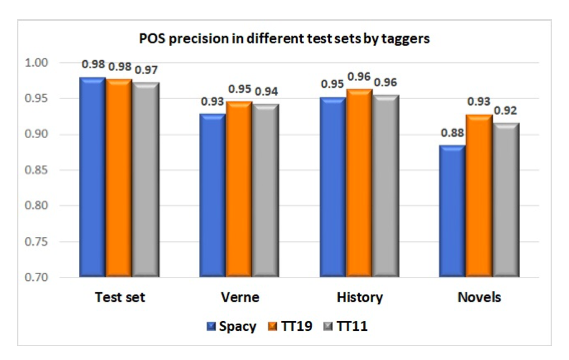
\includegraphics[width=.7\textwidth]{images/pos_tagger.png}
\caption{Preciznost alata za određivanje vrsta reči na različitim skupovima podataka }
\label{Slika}
\end{figure}

\section{Lematizacija}

Proces lematizacije jeste onaj u kome se za svaku reč nalazi njena kanonska forma, tačnije lema. U srpskom jeziku,  za imenice lema je nominativ jednine,  za glagole infinitiv,  a za prideve nominativ jednine muškog roda. Takođe,  proces lematizacije uključuje vraćanje rodne varijacije reči na njen pređašnji oblik. 
Postoje dva metoda za rešavanje problema lematizacije.  Prvi,  da se prema obliku reči otklanja sufiks i nalazi njena lema.  Ovaj oblik rešavanja ne daje tako dobre rezultate.  Drugi pristup uključuje korišćenje skupa podataka koji za svaku reč,  za svaku njenu moguću vrstu reči,  ima određenu lemu.  Postoji mogućnost i kombinovanja ova dva pristupa.  Ovi tekstovi su sakupljani tokom petnaest godina i bilo je mnogo nepravilnosti i nekonzistentnosti koje je trebalo ispraviti. 
Algoritam korišćen u ovom radu za dobijanje vrsta reči je koriščen i za dobijanje lema.  Korišćen je rečnik koji sadrži sve dozvoljene parove vrsta reči i lema za određenu reč.  

Ovaj algoritam nije pravi lematizator,  već na najverovatniju vrstu reči za određenu reč pridruži lemu koja u se nalazi u rečniku.  Zbog ovakov pristupa,  reči koje za istu vrstu reči imaju različite leme ne mogu da postoje u rečniku \cite{tagger}.

Na slici 2.2 je prikazana preciznost 3 različita modela lematizatora trenirana na različitim skupovima podataka.  Slika je preuzeta iz \cite{tagger}.

\begin{figure}[h!]
\centering
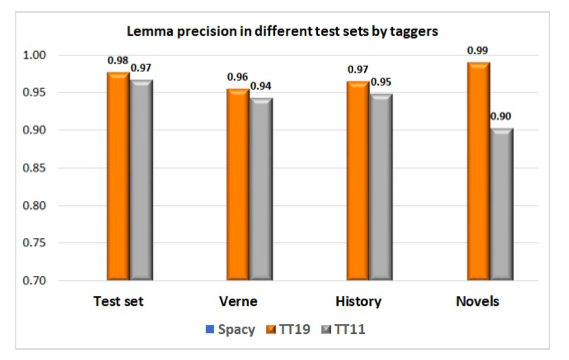
\includegraphics[width=.7\textwidth]{images/lemmatization.png}
\caption{Preciznost lematizatora na različitim skupovima podataka }
\label{Slika}
\end{figure}

\section{Skup podataka pre i nekon obrade}

Skup podataka koji će biti korišćen za eksperimente u ovom radu sadrži sakupljene podatke na već opisan način,  koji su zatim obrađeni pomenutim tehnikama.  Intervjui sa pacijentima obolelim od demencije Alchajmerovog tipa ima 22,  koje nazivamo "pozitivni" i nalaze se u fascikli "P".  Intervjui sa starijim licima koji nemaju utvrđenu demenciju Alchajmerovog tipa ima 57 i oni se nalaze u fascikli "N", a nazivamo ih "negativni".  Nakon procesa određivanja vrsta reči i lema za svaku reč intervjua,  za svaki transkript je kreiran novi dokument koji u sebi sadrzi potrebne informacije.  Ako se u transkriptu nalazi rečenica:
\newline

\noindent\fbox{%
    \parbox{\textwidth}{%
      Ja sam Bojana.  
    }%
}
\newline\newline
Onda će se u odgovarajućoj datoteci naći i sledeći redovi, gde u svakom prva reč označava izvorni oblik reči, druga vrstu, a treća lemu. 
\newline

\noindent\fbox{%
    \parbox{\textwidth}{%
      Ja	ADV	Ja\newline
	sam	AUX	jesam\newline
	Bojana	PROPN	Bojana\newline
	.	PUNCT	.
    }%
}

\section{Vektorska reprezentacija teksta}
\subsection{Vreća reči}
VRećca rečo
\subsection{N-grami}
\subsection{TF metrika}
\subsection{TF-IDF metrika}
\subsection{Naivni Bajesov algoritam}

\chapter{Problem klasifikacije}

\chapter{Rešavanje problema metodama lingvističke analize}

Lingvistička analiza predstavlja pokušaj da računar zaključuje na osnovu značenja taksta i tada kažemo da se sprovodi obrada prirodnog jezika (eng. Natrual Language Processing).  Da bi računar razumeo pisani tekst,  prvo je neophodno podeliti ga na rečenice.  Mnogi lingvistički alati se baziraju na analizi jedne po jedne rečenice.  Zatim se izvodi proces tokenizacije,  deljenja rečenice na pojedinačne reči.  Nakon toga je se izvodi korak lematizacije,  prevođenja svake reči u njen osnovi oblik, tačnije lemu.  U nekim slučajevima,  ovaj korak obukvata i čišćenje, tačnije ispravljanje pogrešno napisanih reči.  Poslednji korak je dodeljivanje vrsta reči svakoj od njih (eng. Part of speech tagging). 
Pacijenti oboleli od Alchajmerove bolesti kao jedan od simptoma imaju gubitak sposobnosti funkcionalne komunikacije i probleme u lingvističkim veštinama.  Procenjivanje afazije kod pacijenata obolelih od demencije Alzhajmerovog tipa je vrlo zahtevan zadatak.  Koristeći različite metrike nad vrstama reči koje su dobijene iz spontanog govora obolelih,  pokušavamo da pronađemo pravilnost i da tako dođemo do zaključaka i mogućnosti klasifikacije na obolele i zdrave pojedince.  
U mnogim naučnim radovima koji se bave temom Alchajmerove bolesti se predstavljaju upravo lingvističke mere kao način razlikovanja obolelih od zdravih pojedinaca i metod za uočavanje pravilosti u njihovom govoru. Potrebno je naći pravilnost u načinu na koji pojedinac govori i koristi svoj vokabular, koliko često izgovara neke vrste reči,  koliko su dugačke rečenice.  Neki od primera korišćenja ovih mera se mogu naći u radovima , \cite{automaticdetandrat}, \cite{Evaloftechfolexicalperformance} i \cite{linguisticfeatures}.

\section{Lingvističke mere}

Korišćeno je ukupno šesnaest mera u okviru ovog rada.  Mere bazinare na vrstama reči uključuju frekvenciju pojavljivanja određene vrste reči u tekstu, kao i tu vrednost normalizovanu ukupnim brojem reči u tekstu. Takođe,  koriste se tri mere Odnos tipa tokena (eng.  Type Token Ratio),  Brunetova statistika (eng. Brunet's Statistic) i Honoreva statistika (eng.  Honore's Statistic) koje počivaju na bogatstvu vokabulara. 
Za svaki tekst se izračunava dužina teksta(N) kao broj izgovorenih reči i prosečna dužina izgovorenih reči.  Vokabular(V) je mera koja pokazuje koliko različitih reči se pojavljuje u tekstu koji se obrađuje.  Vokabular reči izgovorenih jednom (V\textsubscript{1}) se izračunava tako što se od reči koje se nalaze u vokabularu broje samo one koje su izgovorene jednom.  Ove mere se koriste kako samostalno, tako i za izračunavanje mera koje počivaju na bogatstvu vokabulara. 
\break

\section{Mere bazirane na vrstama reči}

Mera pojavljivanja pojedinačne vrste reči u tekstu se izračunava tako što se broji svako pojavljivanje te vrste reči.  Pored toga,  izračunavamo i frekvencije pojavljivanja različitih vrsta reči normalizovane ukupnim brojem reči u tekstu.  U okviru ovog rada, razmatrane su mere vezane količinu imenica,  glagola,  prideva, priloga i zamenica kao i njihove normalizovane vrednosti.  Od koristi mogu biti i odnosi između ovih vrednosti, pa se tako izračunavaju i odnos između količine pojavljivanja imenica i glagola,  zamenica i imenica i zamenica i glagola.  (TODO: Proveriti i ostale, sa pridevima npr.) Ove mere su izabrane heuristički i predstavljaju leksičku raspodeljenost izgovorenih reči.  
Količina imenica pokazuje sposobnost ispitanika da koristi imenice i ona bi mogla biti osetljiva na probleme sa pronalaženjem reči od čega pate osobe koje imaju Alchajmerovu bolest. Količina zamenica je u konstrastu sa količinom imenica i koristi se kao merilo indirektnog referenciranja.  Količina prideva prikazuje kvalitet govora obolele osobe, tačnije mogućnost za opisivanjem. Količina glagola se često koristi kao lingvistička mera i meri tečnost govora. \cite{Evaloftechfolexicalperformance}.  Ove mere su korišćene u mnogim prethodnim istraživanjima kao što su \cite{automaticdetandrat}, \cite{Evaloftechfolexicalperformance} i \cite{linguisticfeatures}. 

\section{Mere bazirane na bogatstvu vokabulara}
 
Tri mere koje se zasnivaju na bogatstvu vokabulara su: Odnos tipa tokena (eng. Type Token Ratio),  Brunetova statistika (Brunet's Statistic) i Honoreva statistika (Honore's Statistic).  Za njihovo izračunavanje neophodno je prvo izračunati dužinu teksta, bogatstvo vokabulara i bogatstvo vokabulara za reči izrečene jednom.  Dužina teksta se meri kao broj reči koje se pojavljuju u tekstu i označava se sa N.  Mera bogatstva vokabulara se izračunava tako što se broji koliko različitih reči se pojavljuje u tekstu i označava se sa V. Mera bogatstva vokabulara za reči izgovorene jednom se izračunava tako što se broje reči u tekstu koje se pojavljuju samo jednom.  Ova mera se označava sa V\textsubscript{1} .  

\subsection{Odnos tipa tokena}

Odnos tipa tokena (eng. Type Token Ratio) se računa po formuli:

\begin{equation}
	TTR = \frac{V}{N}
\end{equation}

gde je N dužina teksta, a V mera bogatstva vokabulara i predstavlja odnos ove dve vrednosti. Ova mera je osetljiva na dužinu teksta.  Veće vrednosti odnosa tipa tokena se povezuju sa bogatijim vokabularom. 

\subsection{Brunetov Indeks}

Brunetov indeks (eng. Brunet's Statistic) se računa po formuli:

\begin{equation}
	W = N^{V^-0.165}
\end{equation}

gde je N dužina teksta, a V mera bogatstva vokabulara. Ova mera se takođe povezuje sa bogatijim vokabularom, ali nije osetljiva na dužinu teksta.  Tipične vrednosti su između 10 i 20.  Manje vrednosti se povezuju sa bogatijim govorom. 

\subsection{Honoreva Statistika}

Honoreva Statistika (eng. Honore's Statistic) se računa po formuli:

\begin{equation}
	R = \frac{100logN}{1 - \frac{V_1}{V}}
\end{equation}

de je N dužina teksta, a V mera bogatstva vokabulara, a V\textsubscript{1} bogatstvo vokabulara za reči izrečene jednom.  Veće vrednosti se povezuju sa bogatijim govorom.  

\section{Klasifikacija bazirana na lingvističkim merama}

Za izračunavanje mera pomenutih u prethodnim sekcijama,  koje nazivamo lingvističkim,  koriste se već obrađeni podaci u kojima je svakoj reči svakog teksta pridružena njena vrsta.  Izračunavanje mera koristeći tako pripremljene tekstove nije teško.  Mere izračunavamo za svaki tekst pojedinačno u korpusu koji sadrži kako pozitivno, tako i negativno klasifikovane tekstove.  Mere čuvamo u okviru datoteke koja nosi ime ispitanika sa ekstenzijom .txt. Ovakve mere možemo koristiti za upoređivanje i vizuelno prikazivanje na grafikonima. Da bismo procenili koliko je neka od metrika korisna u proceni da li je neko oboleo od Alchajmerove bolesti ili ne,  moramo na osnovu nje pokušati da klasifikujemo novi tekst kao pozitivan ili negativan.  Ova vrsta klasifikacije se naziva binarna klasifikacija. 

Kao prvi korak klasifikacije,  neophodno je podeliti skup podataka za treniranje i za testiranje.  Skup za treniranje se naziva trening skup i služi za kreiranje klasifikatora.  Skup za testiranje se naziva testni skup i služi za evaluaciju klasifikatora. U većini slučajeva testni skup predstavlja manji deo korpusa od trening skupa.  Korak deljenja korpusa na trening i testni skup se naziva stratifikacija \cite{MarijaMR}.   Neophodno je da skupovi budu ravnopravno raspodeljeni.  Oba skupa treba da reprezentuju ceo uzorak koji se razmatra. U svakom skupu treba da se nađe određeni procenat obe klase koje razmatramo.  Korpus delimo na ove dve grupe na osnovu jedne karakteristike koja je izabrana, a u slučaju klasifikacije je najčešće to baš ona karakteristika koja određuje kojoj klasi uzorak pripada.  U slučaju klasifikacije obolelih od Alchajmera, karakteristika koju biramo je pripadnost pozitivnom i negativnom korpusu, tačnije da li je osoba obolela od Alchajmera ili ne.  

Korak treniranja modela u ovom slučaju je već odrađen, pošto već imamo sve metrike izračunate za trening skup. Vrednosti metrika iz trening skupa ćemo u koraku evaluacije porediti sa vrednostima metrika iz testnog skupa.

Korak evaluacije u ovom slučaju obuhvata procenu kvaliteta klasifikacije za svaku od metrika koje smo pomenuli u prethodnim sekcijama.  Vrednosti metrike za jedan tekst iz testnog skupa poredimo sa svim vrednostima metrika iz trening skupa i prema blizini odlučujemo kom od skupova tekst iz testnog skupa treba da pripadne po našem klasifikatoru. Zatim se klasa poredi sa stvarnom klasom koju tekst nosi. 

Ako pretpostavimo da trening i test skup sadrže sledeće dokumente:

\begin{equation}
	TRENING = {d\textsubscript{1}, d\textsubscript{2}, \textsubscript{3}, \textsubscript{4}}
\end{equation}

\begin{equation}
	TEST = {d\textsubscript{5}}
\end{equation}

gde dokumenti d\textsubscript{1}, i d\textsubscript{2} pripadaju skupu P,  a dokumenti \textsubscript{3}, i \textsubscript{4} skupu N, a d\textsubscript{5} pripada skupu P

i da radimo klasifikaciju po metrici X, onda sledi izračunavanje:

\begin{align}
	y\textsubscript{1} = \text{abs}(\text{X}(d\textsubscript{1}) - \text{X}(d\textsubscript{5})) \\
	y\textsubscript{2} = \text{abs}(\text{X}(d\textsubscript{2}) - \text{X}(d\textsubscript{5})) \\
	y\textsubscript{3} = \text{abs}(\text{X}(d\textsubscript{3}) - \text{X}(d\textsubscript{5})) \\
	y\textsubscript{4} = \text{abs}(\text{X}(d\textsubscript{4}) - \text{X}(d\textsubscript{5})) \\
	y\textsubscript{P} = y\textsubscript{1} + y\textsubscript{2} \\
	y\textsubscript{N} = y\textsubscript{3} + y\textsubscript{4}
\end{align}
gde (\text{X}(d\textsubscript{i}) predstavlja vrednost metrike X u dokumentu d\textsubscript{i}.

Zatim se porede vrednosti y\textsubscript{P} i y\textsubscript{N}.  Koja vrednost je manja,  smatramo da dokument toj grupi pripada posto je ukupan zbir razlika vrednosti između dokumenta {d\textsubscript{5}} od dokumenta iz te grupe manji.  

Sledeći korak je previđanje pripadnosti klasi pomoću klasifikatora za svaki dokument za metriku X.  Nakon ovog koraka se uz svaki dokument iz test skupa nalaze dve klase,  ona koju znamo da je tačna i ona dodeljena klasifikatorom.  Svaki dokument može biti ispravno i neispravno klasifikovan i prema tome može biti u skupu:

\begin{enumerate}
\item Stvarno pozitivni SP (eng. True Positives, TP)
\item Lažno pozitivni LP (eng.  False Positives,  FP)
\item Stvarno negativni SN (eng.  True Negative, TP)
\item Lažno negativni LN (eng.  False Negative, FN)
\end{enumerate}


gde je stvarno pozitivni broj instanci koje su zaista pozitivne i koje je klasifikator označio kao pozitivne.  Lažno pozitivni je broj instanci koje su negativne, a koje je klasifikator označio kao pozitivne.  

Stvarno negativni je broj instanci koje su negativne,  a koje je klasifikator označio kao negativne.  Lažno negativni je broj instanci koje su pozitivne, a koje je klasifikator označio kao negativne.  Njihov zbir treba da bude jednak broju instanci u testnom skupu.  Ova četiri podatka definišu matricu konfuzije (eng. confusion matrix).  Matrica konfuzije je NxN matrica koja se koristi za evaluaciju klasifikacionog modela,  gde je N broj klasifikacionih klasa.  U slučaju višeklasne klasifikacije element matrice Ctextsubscript{ij} predstavlja broj elemenata koji pripadaju klasi i, a klasifikovani su u klasu j \cite{MarijaMR}.  Model je bolji što je više elemenata van dijagonale u matrici jednako nula.  Matrica konfuzije za binarnu klasifikaciju je prikazana na slici 3.1.

\begin{figure}[h!]
\centering
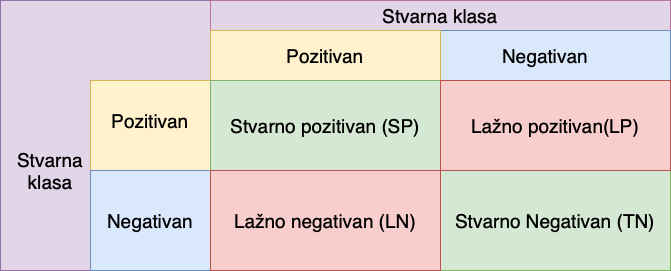
\includegraphics[width=.7\textwidth]{images/confusionMatrix.png}
\caption{Matrica konfuzije}
\label{Slika}
\end{figure}

Ove podatke koristimo za procenu koliko je model dobro istreniran pomoću određenih mera, a neke od njih su sledeće:

\begin{enumerate}
\item Tačnost klasifikacije
\item Preciznost klasifikacije
\item Odziv klasifikacije
\item F-mera
\end{enumerate}

Tačnost klasifikacije (eng.  accuracy ) prikazuje odnos tačno klasifikovanih instanci i svih klasifikovanih instanci i računa se po formuli:

\begin{equation}
	acc = \frac{SP+SN}{SP+SN+LP+LN}
\end{equation}

Preciznost klasifikacije (eng. precision) prikazuje odnos pozitivnih instanci koje su tako klasifikovane i svih instanci koje su klasifikovane pozitivno i računa se po formuli:

\begin{equation}
	P = \frac{SP}{SP+LP}
\end{equation}

Ova mera pokazuje koliko je instanci pogrešno klasifikovano kao pozitivno.  Ako model nema lažnih pozitiva (LP),  onda će vrednost preciznosti biti 1, tačnije 100\%. Što više lažnih pozitiva ima, to že preciznost biti lošija. Vrednosti preciznosti se kreću između 0 i 1. 

Odziv klasifikacije (eng. recall) je mera koja prikazuje odnos pozitivnih instanci koje su tako klasifikovane i zbira pozitivnih instanci koje su tako klasifikovane i pozitivnih instanci koje su klasifikovane kao negativne.  Ova mera se fokusira na broj pozitivnih instanci koje su pogrešno klasifikovane. Ako su sve pozitivne instance upravo tako klasifikovane,  onda će vrednost odziva biti 1, tačnije 100\%. Računa se po formuli:

\begin{equation}
	R = \frac{SP}{SP+LN}
\end{equation}

Preciznost je bitna mera kada nam je bitnija mera lažno pozitivnih od lažno negativnih.  Preciznost je bitna mera u sistemima gde je bitno da se ne dobije negativan rezultat, dok je odziv bitna mera u sistemina gde je problem ako pozitivan slučaj prođe nezapaženo. 

F-mera predstavlja harmonijsku sredinu preciznosti i odziva i razmatra i lažno pozitivne i lažno negativne.  Računa se po sledećoj formuli:

\begin{equation}
	F = \frac{2}{\frac{1}{P} + \frac{1}{R}} = \frac{2 * P * R }{P + R}
\end{equation}

\chapter{Problem klasifikacije}

Problem klasifikacije je jednostavan, od N klasa treba odrediti ispravnu za svaku instancu.  

\chapter{Rešavanje problema Naivnim Bajesovim klasifikatorom}


\chapter{Rešavanje problema metodom podežavajućih vektora}

SVM




Naivni Bajesov model je jedan od probabilističkih modela.  Ovaj algoritam predstavlja jedan od najuspešnijih kada je u pitanju klasifikacija teksta.  Osnovu ovog metoda predstavlja Bajesova teorema koju je predstavio Reverend Thomas Bayes:

\begin{equation}
	P(B|A) = \frac{P(A|B)P(B)}{P(A)}, P(A)>0, P(B)>0
\end{equation}

gde P(B|A) ozna;ava verovatnoću da se desi događaj B pod uslovom da se desio događaj A. 

\chapter{Rezultati}



\chapter{Zaključak}



% ------------------------------------------------------------------------------
% ------------------------------------------------------------------------------

% ------------------------------------------------------------------------------

% ------------------------------------------------------------------------------
% 
% ------------------------------------------------------------------------------
%\literatura

\bibliographystyle{amsplain}
\bibliography{Master_rad}


% ==============================================================================
% Završni deo teze i prilozi
\backmatter
% ==============================================================================


% ------------------------------------------------------------------------------
% Biografija kandidata
\begin{biografija}
  \textbf{Ljubica Peleksić} (\emph{Beograd,
    18.  novembar 1993.}) 
	Ljubicina biografija
\end{biografija}
% ------------------------------------------------------------------------------


\end{document}